
\section{Convexity}
A key property that will enable efficient algorithms is \emph{convexity}.  This comes in the form of \emph{convex sets} and \emph{convex functions}.  Then the constraints to an optimization problem form a  convex set and the objective function is a convex function, then we say that it is a convex optimization problem.

We explain these definitions in the next two subsections.
\subsection{Convex Sets}

\begin{definition}{Convex Combination}{}
Given two points $x,y$, a \emph{convex combination} is any point $z$ that lies on the line between $x$ and $y$.  Algebraically, a \emph{convex combination} is any point $z$ that can be represented as $z = \lambda x + (	1-\lambda) y $ for some multiplier $\lambda \in [0,1]$.
\end{definition}

\begin{figure}[h]
\begin{center}
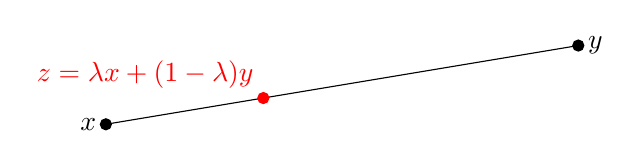
\begin{tikzpicture}

% Define the points
\coordinate (x) at (0,0);
\coordinate (y) at (6,1);
\coordinate (z) at (2/3*0 + 1/3*6, 2/3*0 + 1/3*1);

% Plot the line segment between x and y
\draw (x) -- (y);

% Mark the points with dots and labels
\filldraw [black] (x) circle (2pt) node[anchor=east] {$x$};
\filldraw [black] (y) circle (2pt) node[anchor=west] {$y$};
\filldraw [red] (z) circle (2pt) node[anchor=south east] {$z = \lambda x + (1-\lambda)y$};

\end{tikzpicture}
\end{center}
\caption{A convex combination of the points $x$ and $y$ is given by $z = \lambda x + (1-\lambda)y$ with any $\lambda \in [0,1]$.  Here we demonstrate this using $\lambda = 2/3$.  }
\end{figure}



\begin{definition}{Convex Set}{}
A set $C$ is convex if it contains all convex combinations of points in $C$.  That is, for any $x,y \in C$, it holds that $ \lambda x + (1-\lambda) y \in C$ for all $\lambda \in [0,1]$.
\end{definition}


\begin{figure}[h]
  \begin{subfigure}[b]{0.45\textwidth}
    \centering
    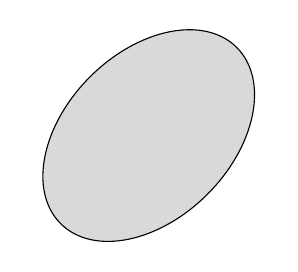
\begin{tikzpicture}
        \draw[rotate=-45,fill=gray!30, thin] (0,0) ellipse (30pt and 45pt);
    \end{tikzpicture}
    \caption{Convex Set}
    \label{a}
  \end{subfigure}
  \begin{subfigure}[b]{0.45\textwidth}
    \centering
    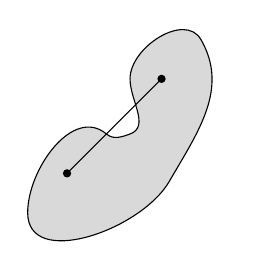
\begin{tikzpicture}
        \useasboundingbox (-1,-1.35) rectangle (1.5,1.35); 
        \draw[fill=gray!30, thin] (0,0) to [out=140,in=90] (-1,-1)
        to [out=-90,in=240] (0.8,-0.6)
        to [out=60,in=-60] (1.2,1.2)
        to [out=120,in=90] (0.3,0.7)
        to [out=-90,in=20] (0.3,0)
        to [out=200,in=-40] (0,0);
        \draw[thin] (-0.5,-0.5) -- (0.7,0.7);
        \fill (-0.5,-0.5) circle[radius=1.5pt];
        \fill (0.7,0.7) circle[radius=1.5pt];
    \end{tikzpicture}
    \caption{Non-convex Set}
    \label{b}
  \end{subfigure}
\end{figure}




%\begin{definition}{Convex Sets}{}
%A set $S$ is \emph{convex} if for any two points in $S$, the entire line segment between them is also contained in $S$.
%That is, for any $x,y \in S$
%$$
%\lambda x + (1-\lambda y) \in S \ \ \text{ for all } \lambda \in [0,1].
%$$
%\end{definition}


    


Examples Convex Sets
\begin{enumerate}
    \item \emph{Hyperplane}  $H = \{x \in \R^n : a^\top x = b\}$
    \item \emph{Halfspace}   $H = \{ x \in \R^n : a^\top x \leq b\}$
    \item \emph{Polyhedron}  $P = \{x \in \R^n : Ax \leq b\}$
    \item \emph{Ball} $S = \{ x \in \R^n : \sum_{i=1}^n x_i^2 \leq 1\}$
    \item \emph{Second Order Cone} $S = \{ (x,t) \in \R^n \times \R : \sum_{i=1}^n x_i^2 \leq t^2 \}$
\end{enumerate}

\begin{example}{Proof that a Polyhedron is Convex}{polyhedron-convex}
Let \( P \) be a polyhedron defined by:
\[ P = \{x \in \mathbb{R}^n : Ax \leq b\} \]
where \( A \) is an \( m \times n \) matrix and \( b \) is an \( m \times 1 \) vector.\\


To prove the convexity of \( P \), we'll use the definition of convexity: For any \( x, y \in P \) and any \( \lambda \in [0,1] \), the point \( z = \lambda x + (1-\lambda) y \) must also belong to \( P \).

Let \( x, y \in P \). Then, by the definition of \( P \), we have:
\[ Ax \leq b \ \ \ \text{ and } \ \ \  Ay \leq b \]

We want to demonstrate the inequality \( Az \leq b \). 
We do this in just a few lines:
\begin{align*}
Az &= A(\lambda x + (1-\lambda) y) & \text{Substituting the expression for \( z \)}\\
&=\lambda Ax + (1-\lambda) Ay & \text{Expanding the matrix-vector product}\\
&\leq \lambda b + (1-\lambda) b & \text{Explaination below}\\
& = b
\end{align*}
The inequality above
uses the fact that \( Ax \leq b \) and \( Ay \leq b \), and since \( \lambda \) is in the interval [0,1], it follows that:
\[ \lambda Ax \leq \lambda b  \ \ \ 
\text{ and } \ \ \ 
(1-\lambda) Ay \leq (1-\lambda) b \]


The computation shows that \( z = \lambda x + (1-\lambda) y \) satisfies \( Az \leq b \) and therefore \( z \in P \).

This shows that the polyhedron \( P \) is convex.
\end{example}

\begin{lemma}{Intersection of Convex Sets is Convex}{}
Let $C_1$ and $C_2$ be convex sets.  Then the intersection $C_1 \cap C_2$ is convex.  
In particular, 
$$C_1 \cap C_2 := \{ x :  x \in C_1 \ \text{ and } x \in C_2\}.
$$
\end{lemma}

\begin{figure}[h]
\begin{center}
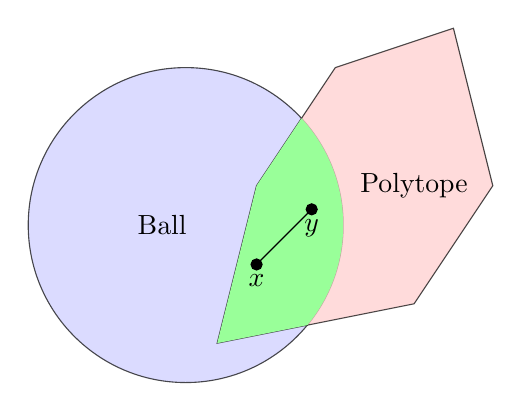
\begin{tikzpicture}

% Draw the circle (ball in 2D) slightly to the left
\filldraw[blue!20, opacity=0.7, draw = black] (0.1,1.5) circle (2cm);

% Draw the 6-vertex polytope slightly to the right
\filldraw[red!20, opacity=0.7, draw = black] (0.5,0) -- (3,0.5) -- (4,2) -- (3.5,4) -- (2,3.5) -- (1,2) -- cycle;

% Shade the intersection
\begin{scope}
  \clip (0.1,1.5) circle (2cm);
  \fill[green!40] (0.5,0) -- (3,0.5) -- (4,2) -- (3.5,4) -- (2,3.5) -- (1,2) -- cycle;
\end{scope}

% Label the circle and polytope
\node at (-0.2,1.5) {Ball};
\node at (3,2) {Polytope};

% Define the points
\coordinate (x) at (1,1);
\coordinate (y) at (1.7,1.7);
\coordinate (z) at (2/3*1 + 1/3*1.7, 2/3*1 + 1/3*1.7);

% Plot the line segment between x and y
\draw (x) -- (y);

% Mark the points with dots and labels
\filldraw [black] (x) circle (2pt) node[anchor=north] {$x$};
\filldraw [black] (y) circle (2pt) node[anchor=north] {$y$};
%\filldraw [red] (z) circle (2pt) node[anchor=south east] {};%$z = \lambda x + (1-\lambda)y$};
\end{tikzpicture}\vspace{1cm}
\end{center}
\caption{The green intersection of the convex sets that are the ball and the polytope is also convex. This can be seen by considering any points $x,y \in \text{Ball} \cap \text{Polytope}$.  Since Ball is convex, the line segment between $x$ and $y$ is completey contained in Ball.  And similarly, the line segment is completely contained in Polytope.  Hence, the line segment is also contained in the intersection.  This is how we can reason that the intersection is also convex.} 
\end{figure}





\section{Convex Functions}


Convex function are "nice" functions that "open up".  They represent an extremely important class of functions in optimization and typically can be optimized over efficiently.



\begin{figure}[H]
    \centering
    \begin{subfigure}[b]{0.45\textwidth}
        \centering
        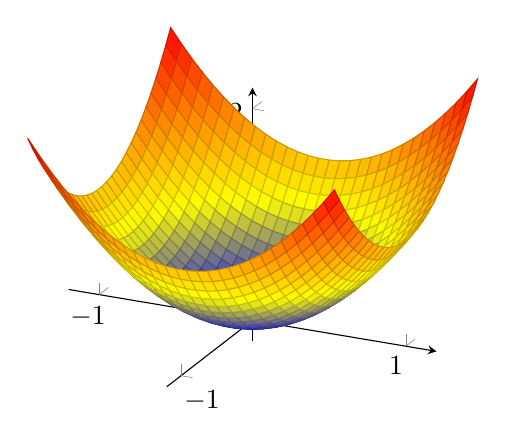
\begin{tikzpicture}[
        declare function = {
            Z(\x,\y) = x^2+y^2;
        }]
        \begin{axis}
           [
           axis lines=center,
           enlargelimits,
           tick align=inside,
           domain=-1:1,
           samples=30, 
           ]
           \addplot3 [surf] {Z(x,y)};
        \end{axis}
        \end{tikzpicture}
        \caption{Convex Function\\ $f(x,y) = x^2 + y^2$.}
    \end{subfigure} 
    \hfill
    \begin{subfigure}[b]{0.45\textwidth}
        \centering
        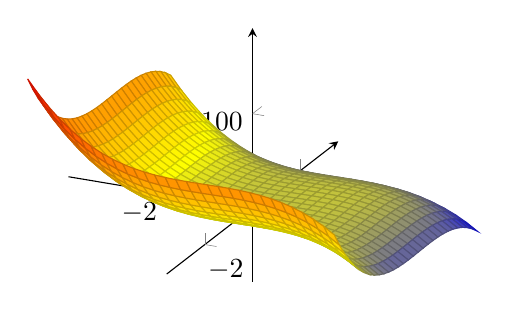
\begin{tikzpicture}[
        declare function = {
            Z(\x,\y) = x^2+y^2- 2*(x - 0.3)^3 - 2*(y - 0.4)^3;
        }]
        \begin{axis}
           [
           axis lines=center,
           enlargelimits,
           tick align=inside,
           domain=-3:3,
           samples=30, 
           ]
           \addplot3 [surf] {Z(x,y)};
        \end{axis}
        \end{tikzpicture}
        \caption{Non-Convex Function\\ $f(x,y) = x^2 + y^2 - 2(x - 0.3)^3 - 2(y - 0.4)^3$.}
    \end{subfigure}
    \caption{Comparison of Convex and Non-Convex Functions.}
\end{figure} 


Informally, a function is convex if whenever you draw a line between two points on the function, that line must be above the function. 


\includefiguresource[Illustration explaining the definition of a convex function.][scale = 1]{tikz/convexity-definition.pdf}
\begin{figure}[H]
\end{figure}
%\footnotetext{\url{https://tex.stackexchange.com/questions/394923/how-one-can-draw-a-convex-function}}

Formally, we can make this definition using the idea of convex combinations.



\begin{definition}{Convex Functions}{}
A function $f \colon \R^n \to \R$ is \emph{convex} if for all $x,y \in \R^n$ and $\lambda \in [0,1]$ we have 
\begin{equation}
\lambda f(x) + (1-\lambda)f(y) \geq f(\lambda x + (1-\lambda) y).
\end{equation}
\end{definition}




An equivalent definition of convex function are through the epigraph.

\begin{definition}{Epigraph}{}
The \emph{epigraph} of $f$ is the set $\{(x,y) : y \geq f(x)\}$.  This is the set of all points "above" the function.
\end{definition}

\begin{theorem}{}{}
$f(x)$ is a convex function if and only if the epigraph of $f$ is a convex set.
\end{theorem}

\includegraphicstatic[scale = 0.7]{epigraph.pdf}\footnotemark

\footnotetext{\url{https://tex.stackexchange.com/questions/261501/function-epigraph-possibly-using-fillbetween}}



\begin{example}{Examples of Convex functions}{}

Some examples are 

\begin{itemize}
\item $f(x) = ax + b$
\item $f(x) = x^2$
\item $f(x) = x^4$
\item $f(x) = |x|$
\item $f(x) = e^x$
\item $f(x) = - \sqrt{x}$ on the domain $[0,\infty)$.
\item $f(x) = x^3$ on the domain $[0,\infty)$.
\item $f(x,y) = 
\sqrt{x^2 + y^2}$
\item $f(x,y) = x^2 + y^2 + x$
\item $ f(x,y) = e^{x+y}$
\item $f(x,y) = e^{x} + e^{y} + x^2+  (3x + 4y)^6$
\end{itemize}

\end{example}






\begin{figure}[H]
\begin{center}
    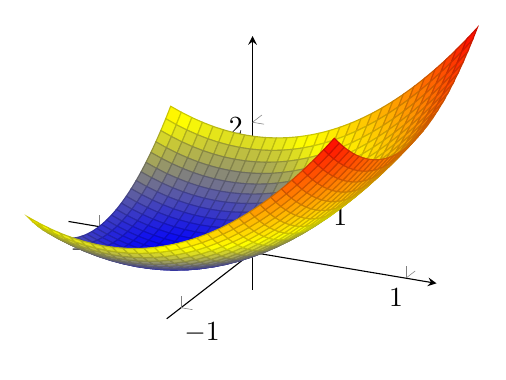
\begin{tikzpicture}[
    declare function = {
        %q(\x) = 5*\x - 1;
        Z(\x,\y) = x^2+y^2 + x; %+ q(\x);
    }]
    \begin{axis}
       [
       axis lines=center,
       enlargelimits,
       tick align=inside,
       domain=-1:1,
       samples=30, 
       %minor tick num=7,
       ]
       \addplot3 [surf] {Z(x,y)};
       %\draw [thick, -latex] (0,0) to [bend right] (0,3);
      % \draw[dashed,line width=0.005\linewidth, ->] (axis cs:-1.1, 1.35, 1) -- (axis cs:0.0,-0.2,0.65);
    \end{axis}
    \end{tikzpicture}
     \hspace{1cm}
    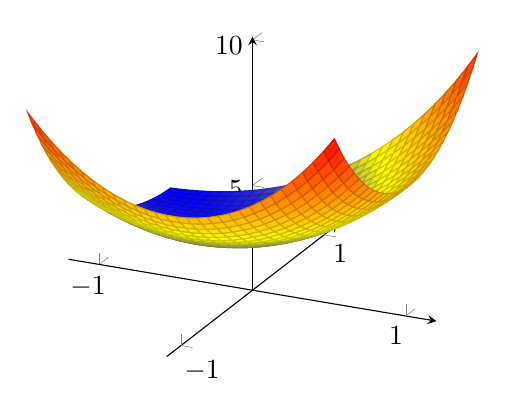
\begin{tikzpicture}[
    declare function = {
        %q(\x) = 5*\x - 1;
        Z(\x,\y) = exp(x+y) + exp(x-y) + exp(-x-y); %+ q(\x);
    }]
    \begin{axis}
       [
       axis lines=center,
       enlargelimits,
       tick align=inside,
       domain=-1:1,
       samples=30, 
       %minor tick num=7,
       ]
       \addplot3 [surf] {Z(x,y)};
       %\draw [thick, -latex] (0,0) to [bend right] (0,3);
      % \draw[dashed,line width=0.005\linewidth, ->] (axis cs:-1.1, 1.35, 1) -- (axis cs:0.0,-0.2,0.65);
    \end{axis}
    \end{tikzpicture}
    \hspace{1cm}
     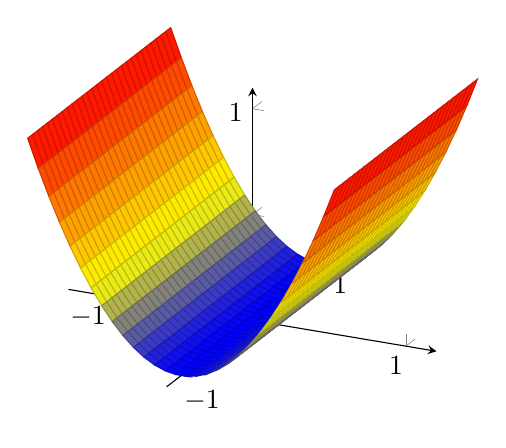
\begin{tikzpicture}[
    declare function = {
        %q(\x) = 5*\x - 1;
        Z(\x,\y) = x^2; %+ q(\x);
    }]
    \begin{axis}
       [
       axis lines=center,
       enlargelimits,
       tick align=inside,
       domain=-1:1,
       samples=30, 
       %minor tick num=7,
       ]
       \addplot3 [surf] {Z(x,y)};
       %\draw [thick, -latex] (0,0) to [bend right] (0,3);
      % \draw[dashed,line width=0.005\linewidth, ->] (axis cs:-1.1, 1.35, 1) -- (axis cs:0.0,-0.2,0.65);
    \end{axis}
    \end{tikzpicture}
\end{center}
    \caption{Convex Functions $f(x,y) = x^2 + y^2+ x$ ,  $f(x,y) = e^{x+y} + e^{x-y} + e^{-x-y} $, and $f(x,y) = x^2 $.}
\end{figure} 





\subsection{Proving Convexity - Characterizations}

\begin{theorem}{Convexity: First order characterization - linear underestimates}{}{}
Suppose that $f\colon \R^n \to \R$ is differentiable.  Then $f$ is convex if and only if for all $\bar x \in \R^n$, then linear tangent is an underestimator to the function, that is,
$$
f(\bar x) + (x - \bar x)^\top \nabla f(\bar x) \leq f(x).
$$
\end{theorem}

\begin{figure}[H]
\begin{center}
\includegraphicstatic[scale = 0.12, trim = {0 0 0 10cm}, clip ]{first-order-convexity}\footnotemark
\end{center}
\end{figure}
\footnotetext{\url{https://machinelearningcoban.com/2017/03/12/convexity/}}



\begin{theorem}{Convexity: Second order characterization - positive curvature}{}
We give statements for uni-variate functions and multi-variate functions.
\begin{itemize}
\item Suppose $f \colon \R \to \R$ is twice differentiable.  Then $f$ is convex if and only if $f''(x) \geq 0$ for all $x \in \R$.
\item Suppose $f \colon \R^n \to \R$ is twice differentiable.  Then $f$ is convex if and only if $\nabla^2 f(x) \succcurlyeq 0$ for all $x \in \R^n$.
\end{itemize}
\end{theorem}


\subsection{Proving Convexity - Composition Tricks}


\begin{general}{Positive Scaling of Convex Function is Convex}{}
If $f$ is convex and $\alpha > 0$, then $\alpha f$ is convex. 

\textcolor{blue}{\textbf{Example: } $f(x) = e^x$ is convex.  Therefore, $25 e^x$ is also convex.}
\end{general}

\begin{general}{Sum of Convex Functions is Convex}{}
If $f$ and $g$ are both convex, then $f+g$ is also convex.

\textcolor{blue}{\textbf{Example: } $f(x) = e^x, g(x) = x^4$ are convex.  Therefore, $e^x + x^4$ is also convex.}
\end{general}

\begin{general}{Composition with affine function}{}
If $f(x)$ is convex, then $f(a^\top x + b)$ is also convex.

\textcolor{blue}{\textbf{Example: } $f(x) = x^4$ are convex.  Therefore, $(3x + 5y + 10z)^4$ is also convex.}
\end{general}

\begin{general}{Pointwise maximum}{}
If $f_i$ are convex for $i=1, \dots, t$, then $f(x) = \max_{i=1, \dots, t} f_i(x)$ is convex.

\textcolor{blue}{\textbf{Example: } $f_1(x) = e^{-x}$, $f_2(x) = e^{x}$ are convex.  Therefore, $f(x) = \max(e^x, e^{-x})$ is also convex.}
\end{general}

\begin{general}{Other compositions}{}
Suppose 
$$
f(x) = h(g(x)).
$$
\begin{enumerate}
\item If $g$ is convex, $h$ is convex and \textbf{non-decreasing}, then $f$ is convex.
\item If $g$ is concave, $h$ is convex and \textbf{non-increasing}, then $f$ is convex.
\end{enumerate}

\textcolor{blue}{\textbf{Example 1: } $g(x) = x^4$ is convex, $h(x) = e^{x}$ is convex and non-decreasing.  Therefore, $f(x) = e^{x^4}$ is also convex.}\\

\textcolor{blue}{\textbf{Example 2: } $g(x) = \sqrt{x}$ is concave (on $[0,\infty)$), $h(x) = e^{-x}$ is convex and non-increasing.  Therefore, $f(x) = e^{-\sqrt{x}}$ is convex on $x \in [0,\infty)$.}
\end{general}
